\documentclass{article}
\usepackage{tabularx}
\usepackage{amsmath}
\usepackage{here}
\usepackage{graphicx}
\usepackage[margin=2cm]{geometry}
\usepackage{cite}
\usepackage[final]{hyperref}
\usepackage{listings}
\hypersetup{
	colorlinks=true,
	linkcolor=blue,
	citecolor=blue,
	filecolor=magenta,
	urlcolor=blue         
}

\begin{document}

\title{Project\\An ant simulation}
\maketitle

\section{Introduction}
The project needs to be sent four days before the final exam. Only the source code and the report are required (no binary code). Please send it to robinfaurypro@gmail.com. In the rapport, you must discuss any technical choices you did. Why you prefer to create a buffer or a surface, why you recompute this value, etc...
The project is an ant simulation. Ants must leave the anthill to find some resources. The only ability they have is to put pheromone on the floor. Thus pheromones can store information like the distance to the anthill or the food.
\begin{figure}[H]
	\centering
	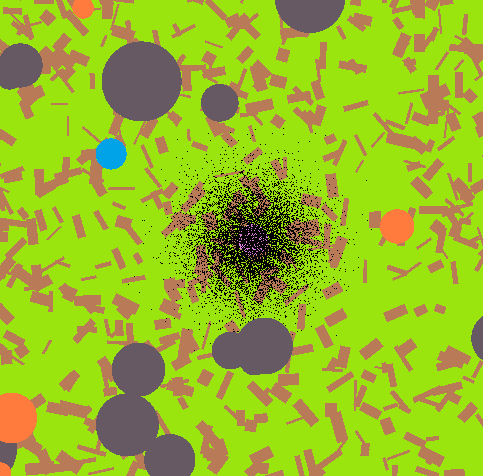
\includegraphics[scale=0.8]{figures/ant.png}
	\caption{The ant simulation}
\end{figure}

The initial code of the project can be find in this git repository:
\begin{lstlisting}
	https://github.com/robinfaurypro/GPGPU_ISIMA_2021-2022.git
\end{lstlisting}

For this simulation, we will use a real time application. The CUDA part will compute the image to show as fast as possible and OpenGL will print this image on the screen. Working with image is more complex than working with buffer. For the moment we use only buffer to keep simple. However, to print on the screen a buffer, we need first to convert it as a texture. A better option is to work directly with texture. GPU texture can be seen in the same way than buffer, but they come with a collection of tool (interpolation, repeat, ...).\\
For this project, we ask OpenGL to generate the texture to show and we use the interop feature to convert it into a surface. Surfaces can be send to the kernel in the same way than buffers. You can create a float4 on the kernel to fill the surface with your color. You can also see how to create a surface CUDA in the exemple (Creation of a surface cuda).
\begin{lstlisting}
	__global__  void kernel_draw_map(cudaSurfaceObject_t surface) {
		int32_t x = blockIdx.x * blockDim.x + threadIdx.x;
		int32_t y = blockIdx.y * blockDim.y + threadIdx.y;
		float4 color = make_float4(0.6f, 0.9f, 0.05f, 1.0f);
		surf2Dwrite(color, surface, x * sizeof(float4), y);
	}
\end{lstlisting}

\section{Drawing the map}
The CUDA languages support the struct keyword. You can create a struct for the rock or the stick or the water and use thus structures in your kernel.
\begin{lstlisting}
	struct Rock {
		float u;
		float v;
		float radius;
	};
\end{lstlisting}
\begin{lstlisting}
	__global__ 
	void kernel_draw_map(cudaSurfaceObject_t surface, Rock* rocks, int32_t nb_rocks)
\end{lstlisting}
Generate a random map by using the std::uniform\_real\_distribution tool. You can create a buffer for each type of object you want in your scene or one big buffer with all of them. In this exemple I choose:
\begin{itemize}
	\item 42 rocks with the color 0.4f, 0.35f, 0.39f, 1.0f
\item 3 water source with the color 0.725f, 0.478f, 0.341f, 1.0f
\item 15 food spot with the color 1.f, 0.478f, 0.241f, 1.0f
\item 2000 sticks with the color 0.725f, 0.478f, 0.341f, 1.0f
\item 1 anthill with the color 0.839f, 0.486f, 0.839f, 1.0f
\end{itemize}

\subsection{Draw a circle}
To draw a circle you can use the hypotf function from CUDA. This function compute the distance between two point. 
\begin{lstlisting}
	if (hypotf(food[i].u - uv.x, food[i].v - uv.y) < food[i].radius) {
		color = FOOD_COLOR;
	}
\end{lstlisting}
For your information, operator can be overridden to create useful function. In this case we can create this one:
\begin{lstlisting}
	__device__ float2 operator-(float2 a, float2 b) {
		return make_float2(a.x - b.x, a.y - b.y);
	};
\end{lstlisting}
You can notice the \_\_device\_\_ keyword to specify the function to the device. This function is accessible only by other device functions or kernel functions.

\subsection{Draw a oriented box}
Oriented box is more difficult to generate. Fortunately, drawing shape is well define right now and you can find useful formulas in this website (https://www.iquilezles.org/www/articles/distfunctions2d/distfunctions2d.htm). Thus content is very often use by people working on shadertoy (https://www.shadertoy.com). If you want to learn more about graphic computing, I recommend you to take a look in detail in the code of some shaders.
\begin{lstlisting}
float OrientedBox( in vec2 p, in vec2 r, float ang ) {
    vec2 w = vec2(cos(ang),sin(ang));

    vec4  q = w.xyyx * p.xxyy;
    vec4  s = w.xyyx * r.xxyy;

    return max(
        max(abs(q.x+q.z)-r.x, abs(q.w-q.y)-r.y ) /
        max(abs(w.x-w.y), abs(w.x+w.y)),
        max(abs(p.x)-max(abs(s.x-s.z),abs(s.x+s.z)),
        abs(p.y)-max(abs(s.y+s.w),abs(s.y-s.w))));
}
\end{lstlisting}
Be careful, this code is in GLSL. You need to convert it into CUDA code if you want to include some stick in your project. The r.xxyy command is equivalent to make\_float4(x, x, y, y).

\begin{figure}[H]
	\centering
	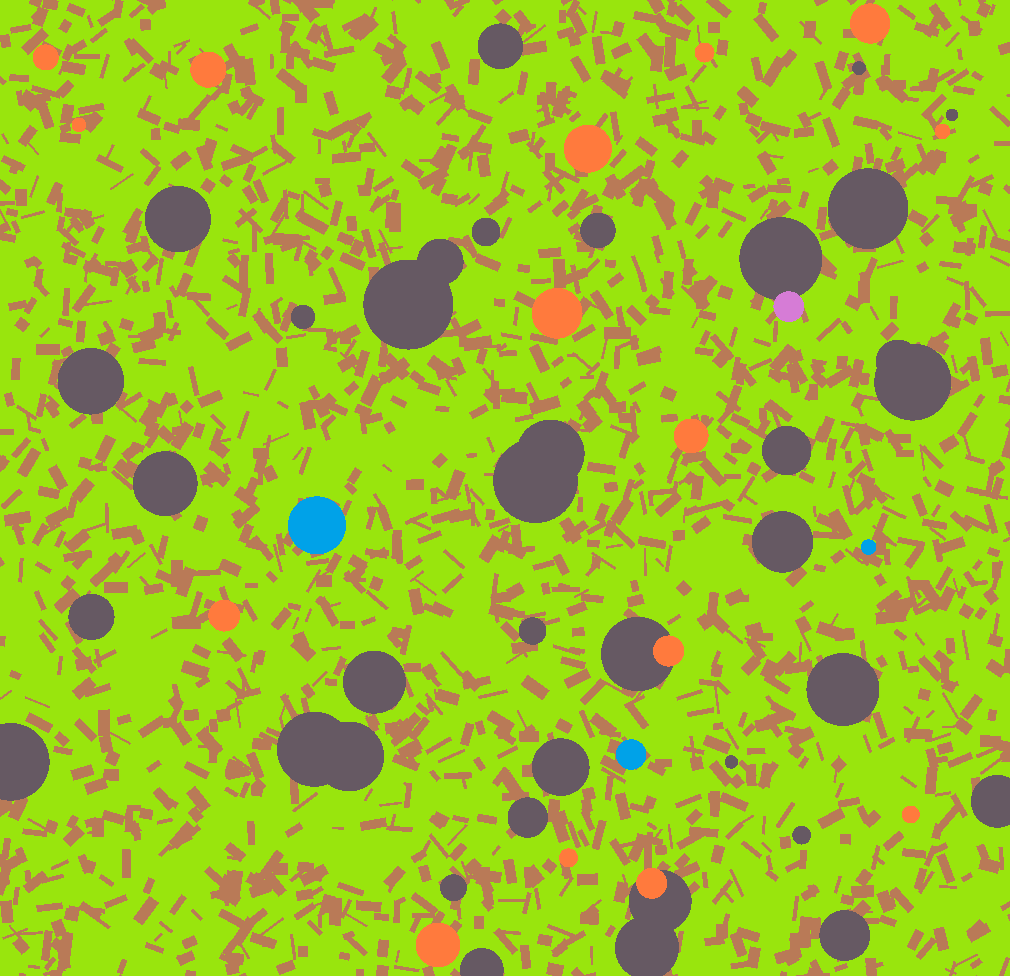
\includegraphics[scale=0.5]{figures/map.png}
	\caption{The map}
\end{figure}

\section{FPS}
If you make the choice to draw the same amount of object in your scene, you need to check the performance of your algorithm. To do so, you need to profile your kernel. A good option is to use the nvprof tool from the CUDA SDK or a custom computation of the Frame Per Second. Most of the time, the FPS are computed simply because it a better metric when you work on a software. Be careful, Drawing the FPS value a lot of time per second will slow down your simulation. A good option is to print it every second in the terminal or in the title of the window.

\section{Ants}
The aim of the ants is to move from the anthill and go to the food or the water and come back when they find some resources. They can go through stick but you cannot walk on rock. One solution can be to find every direction possible (the 8 cases around the ant) and invalid directions that lead to the rock. Moving ants randomly may be the first step to implement. Unfortunately, random in GPGPU is not easy. You can use cuRand to create random number or you can using this formula:
\begin{lstlisting}
__device__ float random(float x, float y) {
	float t = 12.9898f*x + 78.233f*y;
	return abs(fracf(t * sin(t)));
}
\end{lstlisting}
We simply generate a sinus function with a very high frequency and we grab only the absolute value of the fractional part of the result. This give us a number between 0 and 1. The function need a seed generator, the value of u and v are good candidates.

\subsection{Pheromones}
Ants use pheromones to communicate with other ants. A good way to implement it is to create a new surface to store the value of the pheromone. Each ant will send a pheromone with a value of 0.01 and will try to find the strongest pheromone around. For each frame, each value of pheromone will be reduce by 0.0001.
\begin{figure}[H]
	\centering
	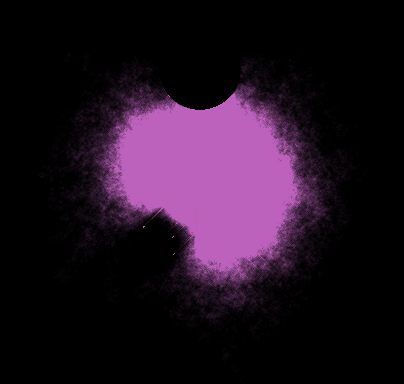
\includegraphics[scale=0.9]{figures/know.png}
	\caption{The known map}
\end{figure}
On of the possible optimization is to use the same kernel to read and write the pheromone map. You don't want to read a value will another thread to currently writing a new value in the same pixel. To avoid this situation you can tell to threads to only read the pixel, synchronize all the threads and then write the new value. The CUDA function to do it is : \_\_syncthreads();

\end{document}